\documentclass{standalone}
\usepackage{tikz}
\usetikzlibrary{patterns, positioning}
\usepackage[sfdefault]{ClearSans} %% option 'sfdefault' activates Clear Sans as the default text font
\usepackage[T1]{fontenc}

\begin{document}
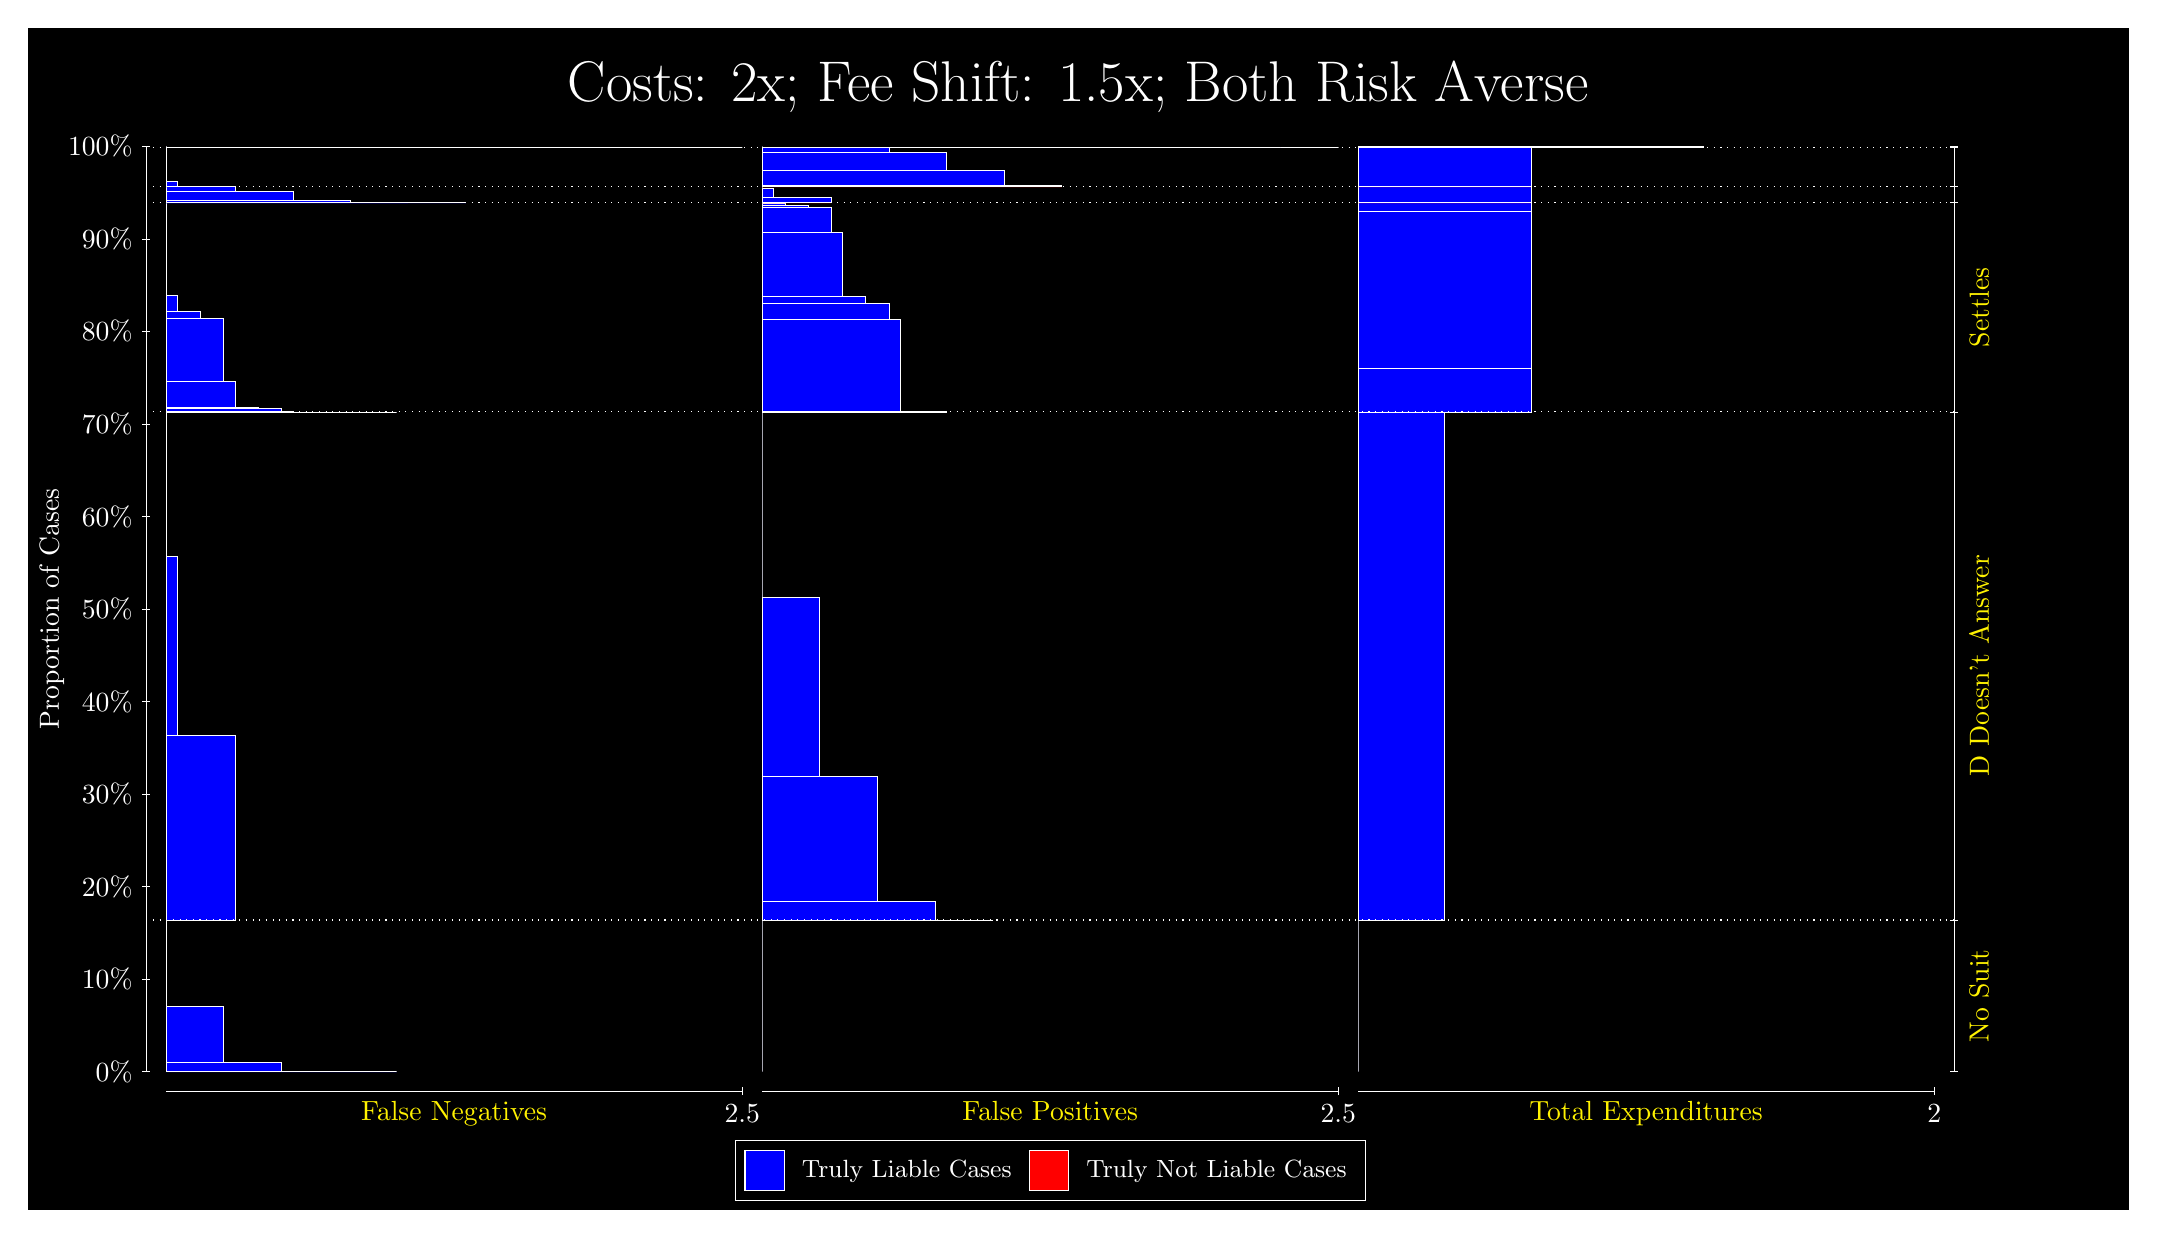
\begin{tikzpicture}
\draw[fill=black] (0,0) rectangle (26.667,15);
\draw[text=white] (0,13.5) rectangle (26.667,15) node[midway] {\huge Costs: 2x; Fee Shift: 1.5x; Both Risk Averse};
\draw[white, very thin] (1.5,1.75) -- (1.5,13.5);
\node[rotate=90, text=white, anchor=center] at (0.3, 7.625) {Proportion of Cases};
\draw[white, very thin] (1.45,1.75) -- (1.55,1.75);
\node[text=white, anchor=east] at (1.45, 1.75) {0\%};
\draw[white, very thin] (1.45,2.925) -- (1.55,2.925);
\node[text=white, anchor=east] at (1.45, 2.925) {10\%};
\draw[white, very thin] (1.45,4.1) -- (1.55,4.1);
\node[text=white, anchor=east] at (1.45, 4.1) {20\%};
\draw[white, very thin] (1.45,5.275) -- (1.55,5.275);
\node[text=white, anchor=east] at (1.45, 5.275) {30\%};
\draw[white, very thin] (1.45,6.45) -- (1.55,6.45);
\node[text=white, anchor=east] at (1.45, 6.45) {40\%};
\draw[white, very thin] (1.45,7.625) -- (1.55,7.625);
\node[text=white, anchor=east] at (1.45, 7.625) {50\%};
\draw[white, very thin] (1.45,8.8) -- (1.55,8.8);
\node[text=white, anchor=east] at (1.45, 8.8) {60\%};
\draw[white, very thin] (1.45,9.975) -- (1.55,9.975);
\node[text=white, anchor=east] at (1.45, 9.975) {70\%};
\draw[white, very thin] (1.45,11.15) -- (1.55,11.15);
\node[text=white, anchor=east] at (1.45, 11.15) {80\%};
\draw[white, very thin] (1.45,12.325) -- (1.55,12.325);
\node[text=white, anchor=east] at (1.45, 12.325) {90\%};
\draw[white, very thin] (1.45,13.5) -- (1.55,13.5);
\node[text=white, anchor=east] at (1.45, 13.5) {100\%};

\draw[white, very thin] (24.457,1.75) -- (24.457,13.5);
\draw[white, very thin] (24.407,1.75) -- (24.507,1.75);
\node[anchor=west] at (24.407, 1.75) {};
\draw[white, very thin] (24.407,3.675) -- (24.507,3.675);
\node[anchor=west] at (24.407, 3.675) {};
\draw[white, very thin] (24.407,10.128) -- (24.507,10.128);
\node[anchor=west] at (24.407, 10.128) {};
\draw[white, very thin] (24.407,12.785) -- (24.507,12.785);
\node[anchor=west] at (24.407, 12.785) {};
\draw[white, very thin] (24.407,12.989) -- (24.507,12.989);
\node[anchor=west] at (24.407, 12.989) {};
\draw[white, very thin] (24.407,13.486) -- (24.507,13.486);
\node[anchor=west] at (24.407, 13.486) {};
\draw[white, very thin] (24.407,13.5) -- (24.507,13.5);
\node[anchor=west] at (24.407, 13.5) {};

\draw[white, very thin, fill=blue] (1.75,1.75) rectangle (4.6775,1.75);
\draw[white, very thin, fill=blue] (1.75,1.75) rectangle (3.9457,1.751);
\draw[white, very thin, fill=blue] (1.75,1.751) rectangle (3.2138,1.8726);
\draw[white, very thin, fill=blue] (1.75,1.8726) rectangle (2.4819,2.579);
\draw[white, very thin, fill=red] (1.75,2.579) rectangle (1.75,2.579);
\draw[white, very thin, fill=blue] (1.75,2.579) rectangle (1.75,3.675);
\draw[white, very thin, fill=blue] (1.75,3.675) rectangle (2.6283,6.0242);
\draw[white, very thin, fill=blue] (1.75,6.0242) rectangle (1.8964,8.2982);
\draw[white, very thin, fill=red] (1.75,8.2982) rectangle (1.75,8.2982);
\draw[white, very thin, fill=blue] (1.75,8.2982) rectangle (1.75,10.128);
\draw[white, very thin, fill=blue] (1.75,10.128) rectangle (4.6775,10.128);
\draw[white, very thin, fill=blue] (1.75,10.128) rectangle (4.3848,10.128);
\draw[white, very thin, fill=blue] (1.75,10.128) rectangle (4.092,10.128);
\draw[white, very thin, fill=blue] (1.75,10.128) rectangle (3.9457,10.128);
\draw[white, very thin, fill=blue] (1.75,10.128) rectangle (3.6529,10.128);
\draw[white, very thin, fill=blue] (1.75,10.128) rectangle (3.3602,10.139);
\draw[white, very thin, fill=blue] (1.75,10.139) rectangle (3.2138,10.168);
\draw[white, very thin, fill=blue] (1.75,10.168) rectangle (2.921,10.181);
\draw[white, very thin, fill=blue] (1.75,10.181) rectangle (2.6283,10.511);
\draw[white, very thin, fill=blue] (1.75,10.511) rectangle (2.4819,11.321);
\draw[white, very thin, fill=blue] (1.75,11.321) rectangle (2.1891,11.408);
\draw[white, very thin, fill=blue] (1.75,11.408) rectangle (1.8964,11.613);
\draw[white, very thin, fill=red] (1.75,11.613) rectangle (1.75,11.613);
\draw[white, very thin, fill=blue] (1.75,11.613) rectangle (1.75,12.785);
\draw[white, very thin, fill=blue] (1.75,12.785) rectangle (5.5558,12.785);
\draw[white, very thin, fill=blue] (1.75,12.785) rectangle (4.8239,12.785);
\draw[white, very thin, fill=blue] (1.75,12.785) rectangle (4.092,12.81);
\draw[white, very thin, fill=blue] (1.75,12.81) rectangle (3.3602,12.923);
\draw[white, very thin, fill=blue] (1.75,12.923) rectangle (2.6283,12.989);
\draw[white, very thin, fill=red] (1.75,12.989) rectangle (1.75,12.989);
\draw[white, very thin, fill=blue] (1.75,12.989) rectangle (2.6283,12.989);
\draw[white, very thin, fill=blue] (1.75,12.989) rectangle (1.8964,13.053);
\draw[white, very thin, fill=red] (1.75,13.053) rectangle (1.75,13.053);
\draw[white, very thin, fill=blue] (1.75,13.053) rectangle (1.75,13.486);
\draw[white, very thin, fill=blue] (1.75,13.486) rectangle (9.0689,13.486);
\draw[white, very thin, fill=blue] (1.75,13.486) rectangle (8.337,13.486);
\draw[white, very thin, fill=blue] (1.75,13.486) rectangle (7.6051,13.486);
\draw[white, very thin, fill=blue] (1.75,13.486) rectangle (6.8732,13.489);
\draw[white, very thin, fill=blue] (1.75,13.489) rectangle (6.1413,13.493);
\draw[white, very thin, fill=blue] (1.75,13.493) rectangle (5.4094,13.494);
\draw[white, very thin, fill=blue] (1.75,13.494) rectangle (3.0674,13.494);
\draw[white, very thin, fill=blue] (1.75,13.494) rectangle (2.3355,13.494);
\draw[white, very thin, fill=red] (1.75,13.494) rectangle (1.75,13.494);
\draw[white, very thin, fill=blue] (1.75,13.494) rectangle (1.75,13.5);
\draw[white, very thin, fill=red] (9.3189,1.75) rectangle (9.3189,1.75);
\draw[white, very thin, fill=blue] (9.3189,1.75) rectangle (9.3189,3.675);
\draw[white, very thin, fill=red] (9.3189,3.675) rectangle (12.246,3.675);
\draw[white, very thin, fill=blue] (9.3189,3.675) rectangle (12.246,3.677);
\draw[white, very thin, fill=blue] (9.3189,3.677) rectangle (11.515,3.9094);
\draw[white, very thin, fill=blue] (9.3189,3.9094) rectangle (10.783,5.5048);
\draw[white, very thin, fill=blue] (9.3189,5.5048) rectangle (10.051,7.7787);
\draw[white, very thin, fill=blue] (9.3189,7.7787) rectangle (9.3189,10.128);
\draw[white, very thin, fill=red] (9.3189,10.128) rectangle (11.661,10.128);
\draw[white, very thin, fill=blue] (9.3189,10.128) rectangle (11.661,10.134);
\draw[white, very thin, fill=red] (9.3189,10.134) rectangle (11.368,10.134);
\draw[white, very thin, fill=blue] (9.3189,10.134) rectangle (11.368,10.14);
\draw[white, very thin, fill=red] (9.3189,10.14) rectangle (11.075,10.14);
\draw[white, very thin, fill=blue] (9.3189,10.14) rectangle (11.075,11.3);
\draw[white, very thin, fill=blue] (9.3189,11.3) rectangle (10.929,11.505);
\draw[white, very thin, fill=blue] (9.3189,11.505) rectangle (10.636,11.592);
\draw[white, very thin, fill=blue] (9.3189,11.592) rectangle (10.344,12.403);
\draw[white, very thin, fill=blue] (9.3189,12.403) rectangle (10.197,12.732);
\draw[white, very thin, fill=blue] (9.3189,12.732) rectangle (9.9044,12.745);
\draw[white, very thin, fill=blue] (9.3189,12.745) rectangle (9.6116,12.774);
\draw[white, very thin, fill=blue] (9.3189,12.774) rectangle (9.4652,12.785);
\draw[white, very thin, fill=blue] (9.3189,12.785) rectangle (9.3189,12.785);
\draw[white, very thin, fill=red] (9.3189,12.785) rectangle (10.197,12.785);
\draw[white, very thin, fill=blue] (9.3189,12.785) rectangle (10.197,12.851);
\draw[white, very thin, fill=blue] (9.3189,12.851) rectangle (9.4652,12.964);
\draw[white, very thin, fill=blue] (9.3189,12.964) rectangle (9.3189,12.989);
\draw[white, very thin, fill=red] (9.3189,12.989) rectangle (13.125,12.989);
\draw[white, very thin, fill=blue] (9.3189,12.989) rectangle (13.125,13.001);
\draw[white, very thin, fill=blue] (9.3189,13.001) rectangle (12.393,13.19);
\draw[white, very thin, fill=blue] (9.3189,13.19) rectangle (11.661,13.422);
\draw[white, very thin, fill=blue] (9.3189,13.422) rectangle (10.929,13.485);
\draw[white, very thin, fill=blue] (9.3189,13.485) rectangle (10.197,13.486);
\draw[white, very thin, fill=red] (9.3189,13.486) rectangle (16.638,13.486);
\draw[white, very thin, fill=blue] (9.3189,13.486) rectangle (16.638,13.486);
\draw[white, very thin, fill=red] (9.3189,13.486) rectangle (15.906,13.486);
\draw[white, very thin, fill=blue] (9.3189,13.486) rectangle (15.906,13.486);
\draw[white, very thin, fill=red] (9.3189,13.486) rectangle (15.174,13.486);
\draw[white, very thin, fill=blue] (9.3189,13.486) rectangle (15.174,13.486);
\draw[white, very thin, fill=red] (9.3189,13.486) rectangle (14.442,13.486);
\draw[white, very thin, fill=blue] (9.3189,13.486) rectangle (14.442,13.489);
\draw[white, very thin, fill=blue] (9.3189,13.489) rectangle (13.71,13.492);
\draw[white, very thin, fill=blue] (9.3189,13.492) rectangle (12.978,13.492);
\draw[white, very thin, fill=blue] (9.3189,13.492) rectangle (12.246,13.492);
\draw[white, very thin, fill=blue] (9.3189,13.492) rectangle (11.515,13.492);
\draw[white, very thin, fill=red] (9.3189,13.492) rectangle (9.3189,13.492);
\draw[white, very thin, fill=blue] (9.3189,13.492) rectangle (9.3189,13.5);
\draw[white, very thin, fill=red] (16.888,1.75) rectangle (16.888,1.75);
\draw[white, very thin, fill=blue] (16.888,1.75) rectangle (16.888,3.675);
\draw[white, very thin, fill=red] (16.888,3.675) rectangle (17.986,3.675);
\draw[white, very thin, fill=blue] (16.888,3.675) rectangle (17.986,10.128);
\draw[white, very thin, fill=red] (16.888,10.128) rectangle (19.083,10.128);
\draw[white, very thin, fill=blue] (16.888,10.128) rectangle (19.083,10.681);
\draw[white, very thin, fill=red] (16.888,10.681) rectangle (19.083,10.681);
\draw[white, very thin, fill=blue] (16.888,10.681) rectangle (19.083,12.681);
\draw[white, very thin, fill=red] (16.888,12.681) rectangle (19.083,12.681);
\draw[white, very thin, fill=blue] (16.888,12.681) rectangle (19.083,12.785);
\draw[white, very thin, fill=red] (16.888,12.785) rectangle (19.083,12.785);
\draw[white, very thin, fill=blue] (16.888,12.785) rectangle (19.083,12.989);
\draw[white, very thin, fill=red] (16.888,12.989) rectangle (19.083,12.989);
\draw[white, very thin, fill=blue] (16.888,12.989) rectangle (19.083,13.486);
\draw[white, very thin, fill=red] (16.888,13.486) rectangle (21.279,13.486);
\draw[white, very thin, fill=blue] (16.888,13.486) rectangle (21.279,13.5);
\draw[white, dotted] (1.5,3.675) -- (24.457,3.675);
\draw[white, dotted] (1.5,10.128) -- (24.457,10.128);
\draw[white, dotted] (1.5,12.785) -- (24.457,12.785);
\draw[white, dotted] (1.5,12.989) -- (24.457,12.989);
\draw[white, dotted] (1.5,13.486) -- (24.457,13.486);
\draw[white, very thin] (1.75,1.5) -- (9.0689,1.5);
\node[text=yellow, anchor=north] at (5.4094, 1.5) {False Negatives};
\draw[white, very thin] (9.0689,1.45) -- (9.0689,1.55);
\node[text=white, anchor=north] at (9.0689, 1.45) {2.5};

\draw[white, very thin] (9.3189,1.5) -- (16.638,1.5);
\node[text=yellow, anchor=north] at (12.978, 1.5) {False Positives};
\draw[white, very thin] (16.638,1.45) -- (16.638,1.55);
\node[text=white, anchor=north] at (16.638, 1.45) {2.5};

\draw[white, very thin] (16.888,1.5) -- (24.207,1.5);
\node[text=yellow, anchor=north] at (20.547, 1.5) {Total Expenditures};
\draw[white, very thin] (24.207,1.45) -- (24.207,1.55);
\node[text=white, anchor=north] at (24.207, 1.45) {2};

\node[text=yellow, centered, rotate=90] at (24.777, 2.7125) {No Suit};
\node[text=yellow, centered, rotate=90] at (24.777, 6.9015) {D Doesn't Answer};
\node[text=yellow, centered, rotate=90] at (24.777, 11.457) {Settles};




\draw (12.978300999999998,1.5) node[draw=none] (baseCoordinate) {};
\begin{scope}[align=center]
        \matrix[scale=0.5, draw=white, below=0.5cm of baseCoordinate, nodes={draw}, column sep=0.1cm]{
            \node[rectangle, draw, minimum width=0.5cm, minimum height=0.5cm, fill=blue] {}; &
            \node[draw=none, font=\small, text=white] (B) {Truly Liable Cases}; &
            \node[rectangle, draw, minimum width=0.5cm, minimum height=0.5cm, fill=red] {}; &
            \node[draw=none, font=\small, text=white] (B) {Truly Not Liable Cases}; \\
            };
\end{scope}

\end{tikzpicture}
\end{document}